\section{Generating Disinformation: Capabilities and Safety Filters}
\label{sec:disinformation_generation}

\subsection{Auditing Disinformation Capabilities}
Whereas the first two studies treat LLMs as simulated people, Vykopal et al.~\cite{vykopal2024disinformation} study how readily LLMs produce disinformation. They evaluate 10 LLMs (among them GPT-3 Davinci, ChatGPT, GPT-4, Vicuna, Falcon, Llama-2 and Mistral) on 20 disinformation narratives from five categories: COVID-19, the Russo-Ukrainian war, health, US elections and regional narratives. For every narrative, each model wrote three articles from a title prompt and three from a title-plus-abstract prompt, and 1,200 generated texts were annotated manually, for example for agreement with the narrative, novel arguments and safety warnings. % SOURCE: Vykopal et al. p.1 (10 LLMs, 20 narratives, 1,200 manually evaluated texts), p.2 (five categories), p.3 (Table 2 model list; three articles per prompt type and narrative)

Their overall conclusion is that current LLMs can produce persuasive news-style texts that support harmful false narratives~\cite{vykopal2024disinformation}. % SOURCE: Vykopal et al. p.1 abstract

\subsection{Differences Between Models and ``Bothsideism''}
The models differ strongly in their willingness to be misused~\cite{vykopal2024disinformation}:
\begin{itemize}
    \item \textbf{Weak or missing safety behaviour:} Vicuna and GPT-3 Davinci readily generated disinformation, rarely disagreed with the prompted narrative and produced convincing articles with novel arguments; the authors consider them the most dangerous models in their study. % SOURCE: Vykopal et al. p.4; conclusion p.8 ("seemingly zero safety filters built-in (Vicuna, Davinci)")
    \item \textbf{Safer models:} Falcon and Llama-2 behaved most safely, which shows that models \emph{can} be trained to refuse such requests; ChatGPT behaved safely in some cases but was significantly less safe than Falcon. Safety therefore does not simply follow the line between open and proprietary models. % SOURCE: Vykopal et al. p.4 (ChatGPT less safe than Falcon), p.8 conclusion (Falcon, Llama-2 safer)
    \item \textbf{``Bothsideism'':} some outputs tried to present a balanced view with arguments for and against a false narrative. The authors note that this is not captured well by their evaluation; for well-established facts such false balance can still lend credibility to a disinformation narrative. % SOURCE: Vykopal et al. p.6 ("overly bothsideist behavior"); last clause = interpretation of this paper
\end{itemize}

\subsection{Can the Generated Articles Be Detected?}
Vykopal et al.\ also test existing detectors of machine-generated text on their articles (Figure~\ref{fig:detectors}). ELECTRA-large detectors fine-tuned on the multilingual MULTITuDE benchmark~\cite{macko2023multitude} perform best, with a macro-F1 of up to 0.82, while most off-the-shelf detectors reach between 0.36 and 0.71. The authors add two caveats: the scores use the optimal threshold on their test set and are therefore a theoretical maximum, and several off-the-shelf detectors are badly calibrated for this kind of data~\cite{vykopal2024disinformation}. % SOURCE: Vykopal et al. Table 6 p.8 (0.82 = ELECTRA [ChatGPT]; other detectors 0.36 Grover ... 0.71 detection-longformer), footnote 6 p.8 (theoretical maximum), p.8 (miscalibrated models)
MULTITuDE itself was built to study how such detectors generalise to unseen languages and unseen generators~\cite{macko2023multitude}. % SOURCE: Macko et al. p.1 abstract (74,081 texts, 11 languages, 8 LLMs; generalisation to unseen languages and LLMs)
Detection is thus possible, but it depends on training detectors on the right generators and on careful calibration.

\begin{figure}[t]
\centering
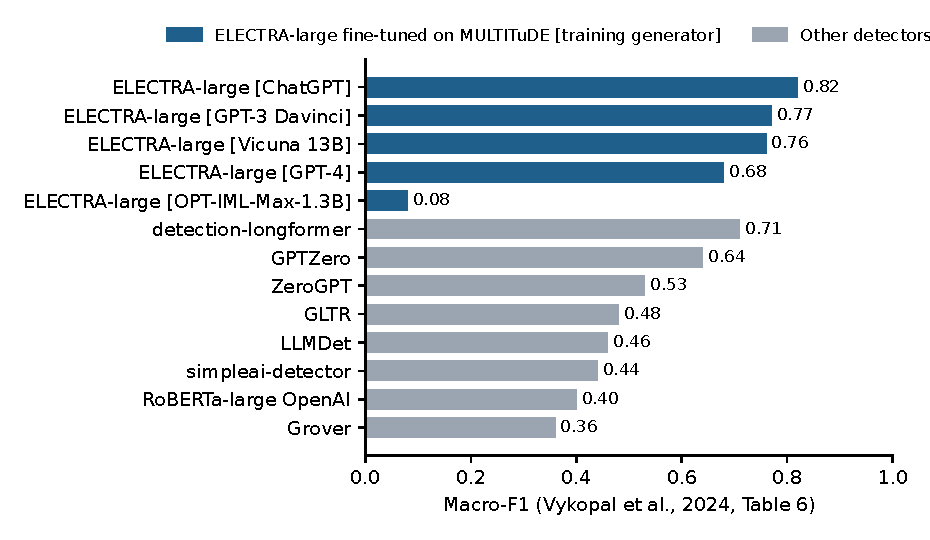
\includegraphics[width=0.95\textwidth]{figures/fig_detectors_paper.pdf}
\caption{Macro-F1 of machine-generated-text detectors on the LLM-generated disinformation articles of Vykopal et al.~\cite{vykopal2024disinformation} (values from their Table~6, optimal threshold per detector). Dark bars: ELECTRA-large fine-tuned on MULTITuDE~\cite{macko2023multitude}, trained on texts of the generator in brackets. Plot made by the author from the published table; no new measurements.}
\label{fig:detectors}
\end{figure}
